
\documentclass[t, 11pt]{beamer}
\pdfmapfile{+sansmathaccent.map}
%%% Работа с русским языком
\usepackage{cmap}				
\usepackage{mathtext} 				
\usepackage[T2A]{fontenc}		
\usepackage[utf8]{inputenc}			
\usepackage[russian, english]{babel}	

\usetheme{Montpellier}
\usecolortheme{beaver} % Цветовая схема



%%% Работа с картинками
\usepackage{graphicx}

\usepackage{csquotes}

\hypersetup{				
	colorlinks=true,       	
	linkcolor=blue,          
	citecolor=black,       
	filecolor=magenta,      
	urlcolor=red           
}
%% табличка
\usepackage{booktabs, caption, makecell}
\usepackage{threeparttable}


\title{Intro to Quantitative methods}
\subtitle{}
\author{Chuvakin Sergey}
\date{\today}
\institute[<<Anthropology>>]{<<School of Advanced Studies>>}

\begin{document}
	
	\frame[plain]{\titlepage}
	\section{lection 2 recap of math}
	
	
	\subsection{Plan}
	\begin{frame} 
		\frametitle{\insertsection} 
		\frametitle{\insertsubsection} 
		\begin{itemize}
   			\item Quantitative vs Qualitative
   			\item Calculus and Linaer Algebra basics 
   			\item probability theory basics
		\end{itemize}
	\end{frame}
	
\subsection{Quantitative vs Qualitative}
	\begin{frame} 
	\frametitle{\insertsection} 
	\frametitle{\insertsubsection} 
	\begin{enumerate}
		\item type of data
			\begin{itemize}
				\item Surveys 
				\item Polls
				\item Internal statistics
			\end{itemize}
		\item type of question 
		\begin{itemize}
			\item What is the relation?
			\item What is a difference?
			\item How one affects on other?
		\end{itemize}
		\item methods
			\begin{itemize}
				\item Statistical tests 
				\item Regression models (the most important one)
				\item Machine Learning (e.g. clsuter analysis)
			\end{itemize}
	\end{enumerate}
\end{frame}

\subsection{Calculus and Linaer Algebra }
\begin{frame} 
	\frametitle{\insertsection} 
	\frametitle{\insertsubsection} 
	The most important terms:
	\begin{enumerate}
		\item vectors
		\item vector operations
		\item matrix
		\item matrix operations
	\end{enumerate}
\end{frame}

\begin{frame} 
	\frametitle{\insertsection} 
	\frametitle{Vectors} 
	Vector - is element of some vector space. It could be Euclidian, Helbert, Topological and many others.  
	\begin{enumerate}
		\item Begins
		\item Ends
		\item \emph{Direction}
		\item magnitude
	\end{enumerate}
\vspace{1cm}
Notation: $\overline{AB}$ or $\overline{a}$
\end{frame}

\begin{frame} 
	\frametitle{\insertsection} 
	\frametitle{Vector Operations} 
	\begin{enumerate}
		\item Addition
		\item Substraction
		\item Scalar multiplication
		\item Dot product 
	\end{enumerate}

\end{frame}
	
\begin{frame} 
	\frametitle{} 
	\frametitle{} 
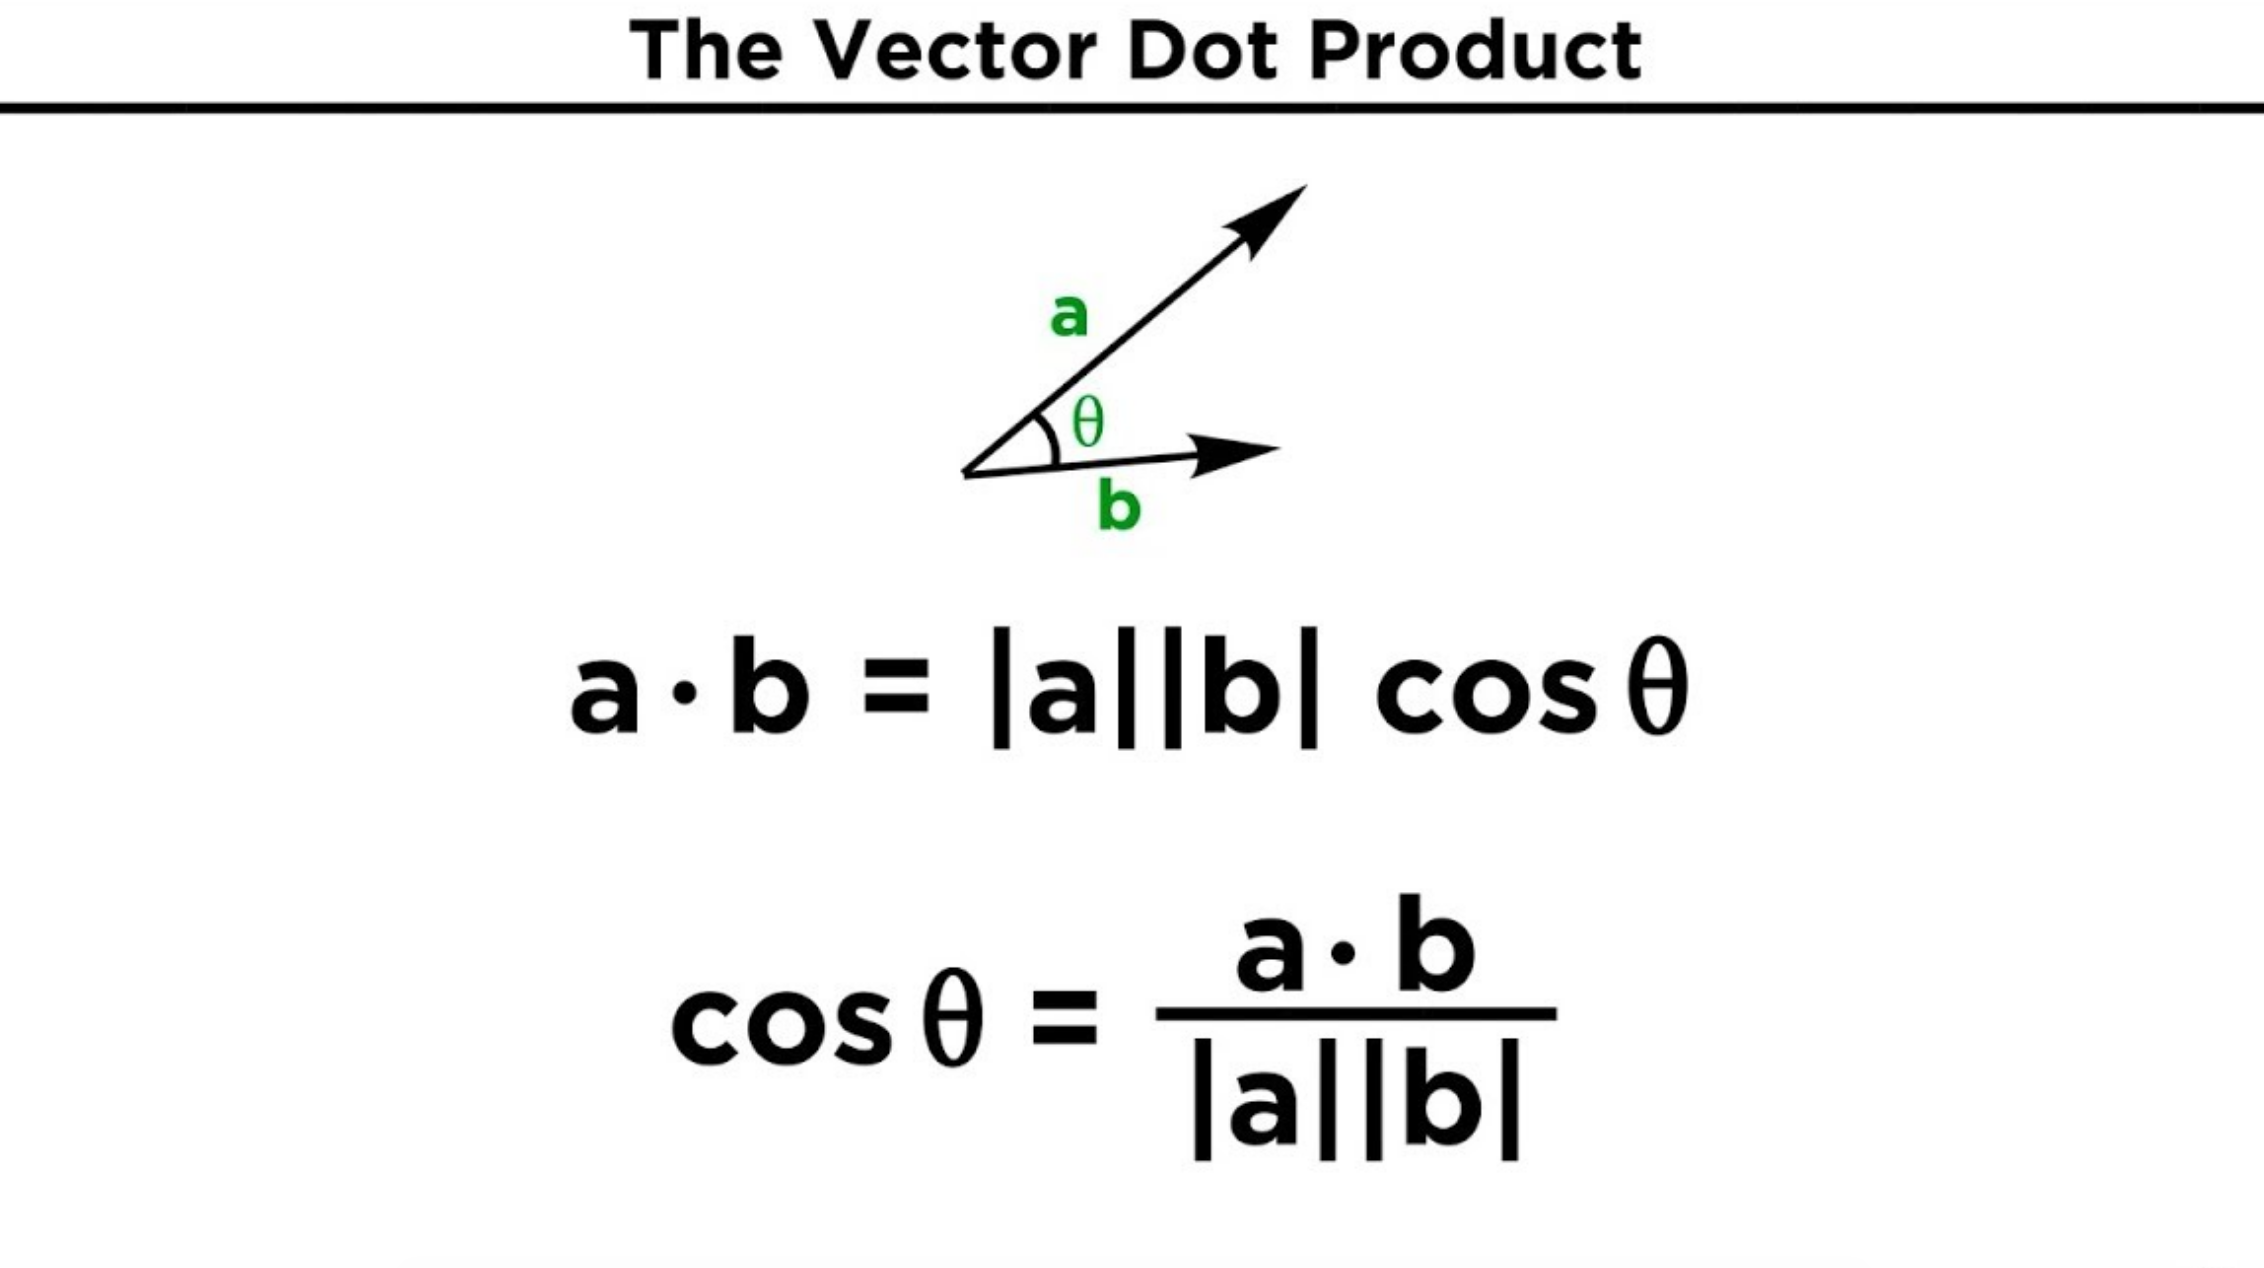
\includegraphics[scale=0.3]{dotprod}	
\end{frame}	

\begin{frame} 
	\frametitle{\insertsection} 
	\frametitle{Vector Operations} 
	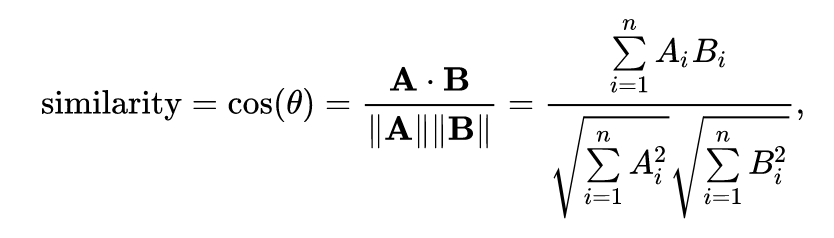
\includegraphics[scale=0.7]{cos}	
\end{frame}	
	
\begin{frame} 
	\frametitle{\insertsection} 
	\frametitle{Matrix} 
	Matrix - set of vectors  
	\begin{enumerate}
		\item Same as vectors
		\item + transposing
		\item Notation (Roman Catholichs)
		\item Dot product 
	\end{enumerate}
	
\end{frame}

\begin{frame} 
	\frametitle{\insertsection} 
	\frametitle{Matices types} 
	Matrix - set of vectors  
	\begin{enumerate}
		\item Row Matrix (aka vector)
		\item Column Matrix (aka vector)
		\item Square Matrix
		\item Rectangular Matrix
		\item Diagonal matrix
		\item Zero or Null Matrix
		\item Unit or Identity Matrix
	\end{enumerate}
\end{frame}

\begin{frame} 
	\frametitle{\insertsection} 
	\frametitle{Dot  Product} 
	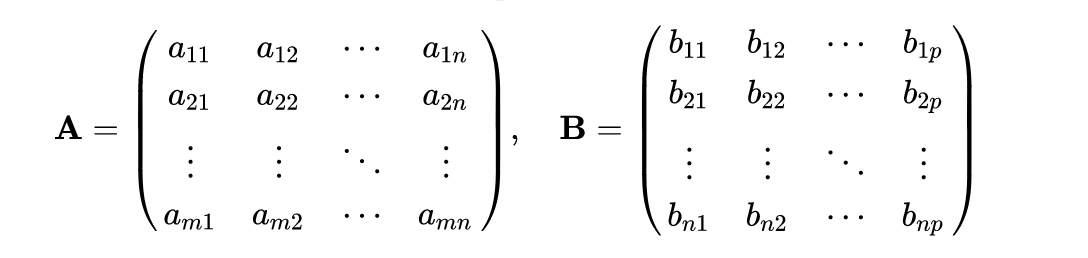
\includegraphics[scale=0.6]{ABmat}	
	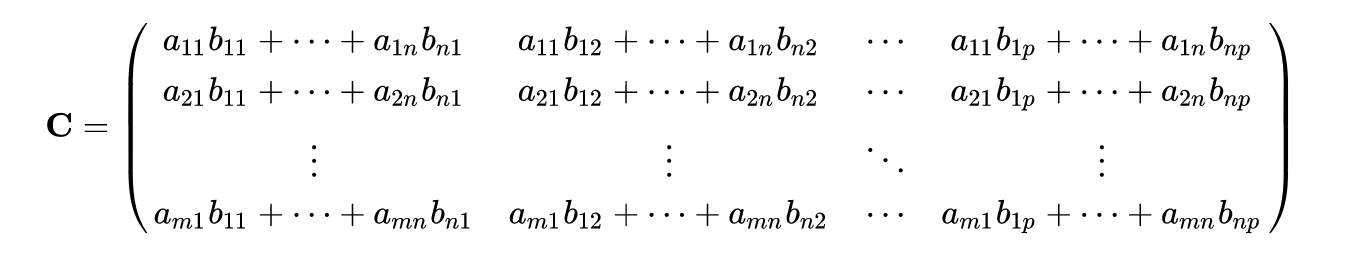
\includegraphics[scale=0.5]{Cmat}	
\end{frame}	

\begin{frame} 
	\frametitle{\insertsection} 
	\frametitle{Dot Product} 
	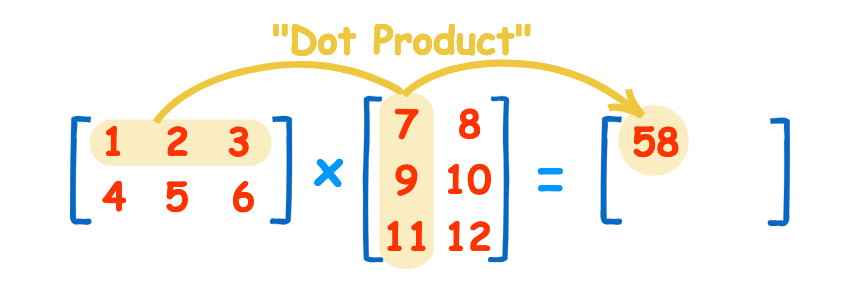
\includegraphics[scale=0.6]{funmath1}	
	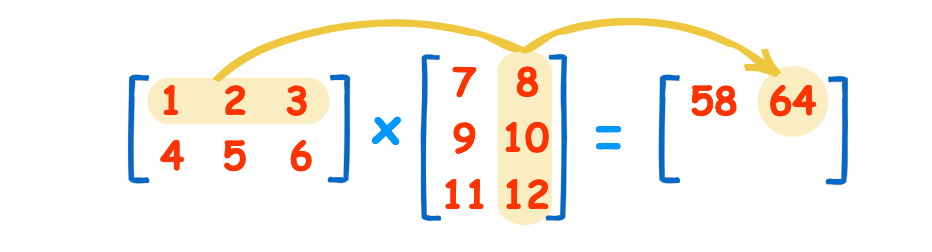
\includegraphics[scale=0.6]{funmath2}	
\end{frame}	

\begin{frame} 
	\frametitle{\insertsection} 
	\frametitle{Dot Product} 
	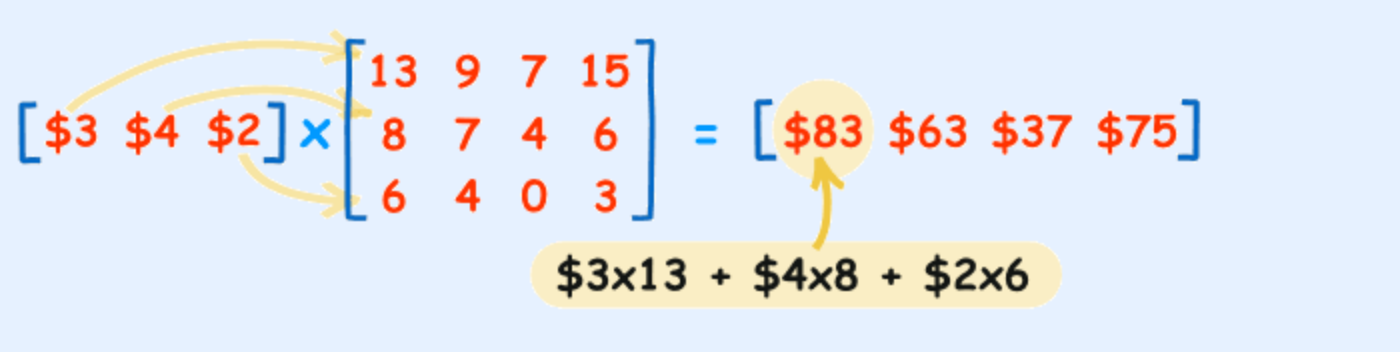
\includegraphics[scale=0.4]{funmath3}	
\end{frame}	

\begin{frame} 
	\frametitle{\insertsection} 
	\frametitle{Dot Product} 
	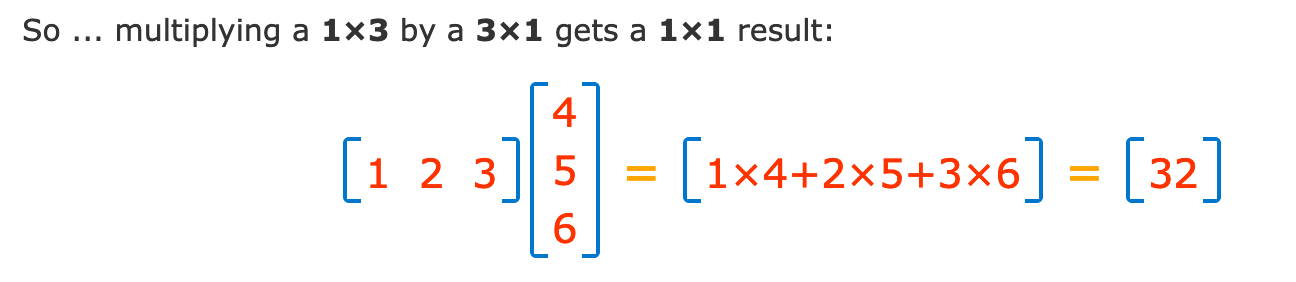
\includegraphics[scale=0.5]{funmath4}	
	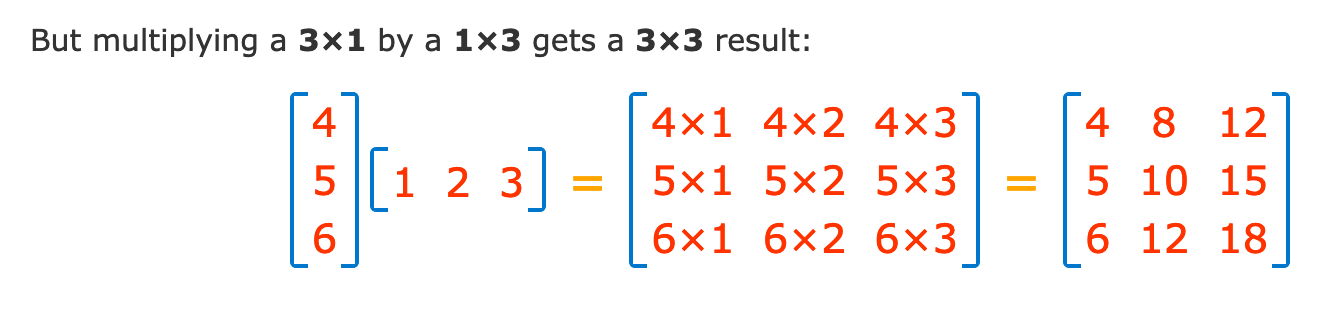
\includegraphics[scale=0.5]{funmath5}	
\end{frame}	

\subsection{Probability basics}
\begin{frame} 
	\frametitle{\insertsection} 
	\frametitle{\insertsubsection} 
	The most important terms:
	\begin{enumerate}
		\item Probability
		\item Independent Events 
		\item Dependent Events
		\item Conditional 
		\item Bayes
	\end{enumerate}
\vspace{1cm}
Notation: $P(A)$ or $P(A|B)$
\end{frame}

\begin{frame} 
	\frametitle{} 
	\frametitle{} 
	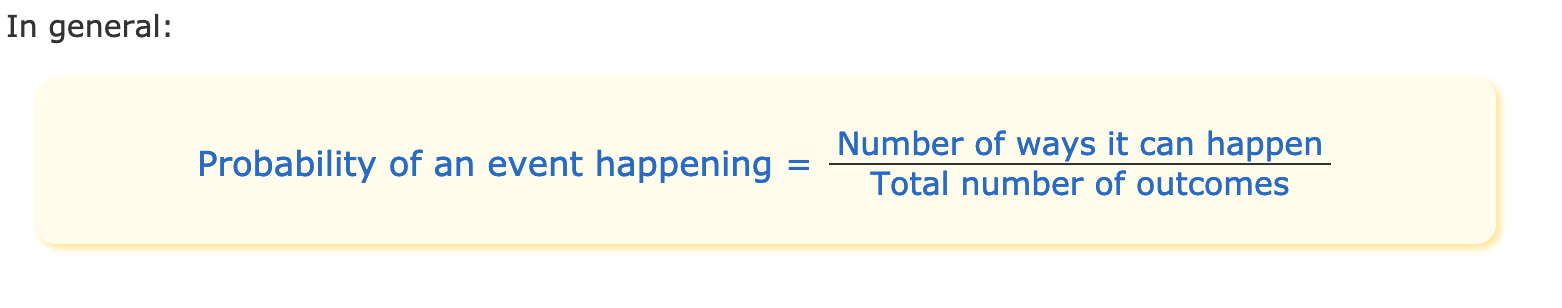
\includegraphics[scale=0.4]{prob}	
	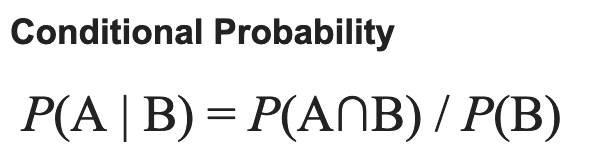
\includegraphics[scale=0.6]{cond}	
\end{frame}	

\begin{frame} 
	\frametitle{} 
	\frametitle{} 
	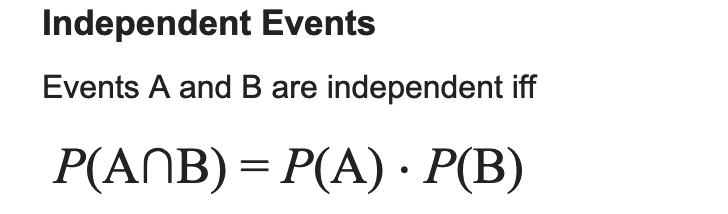
\includegraphics[scale=0.6]{and_prob}	
	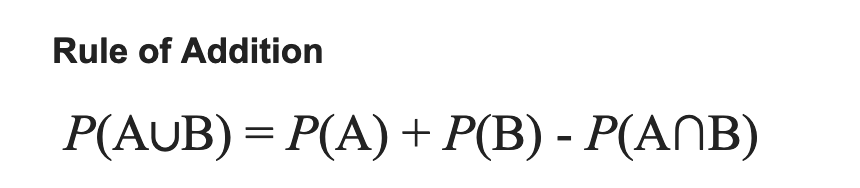
\includegraphics[scale=0.6]{or_prob}	
\end{frame}	

\begin{frame} 
	\frametitle{} 
	\frametitle{} 
	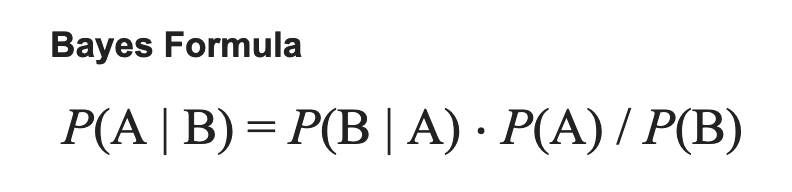
\includegraphics[scale=0.6]{Bayes}	
\end{frame}	

\end{document}
